\subsection{Estrutura do trabalho} \label{subsec:estrutura}

 Este documento está estruturado em~\ref{sec:conclusoes} capítulos, divididos da seguinte forma:
   
    \begin{figure}[H]
    	\centering
    	\caption{Estrutura da dissertação}
    	\label{fig:estrutura}
    	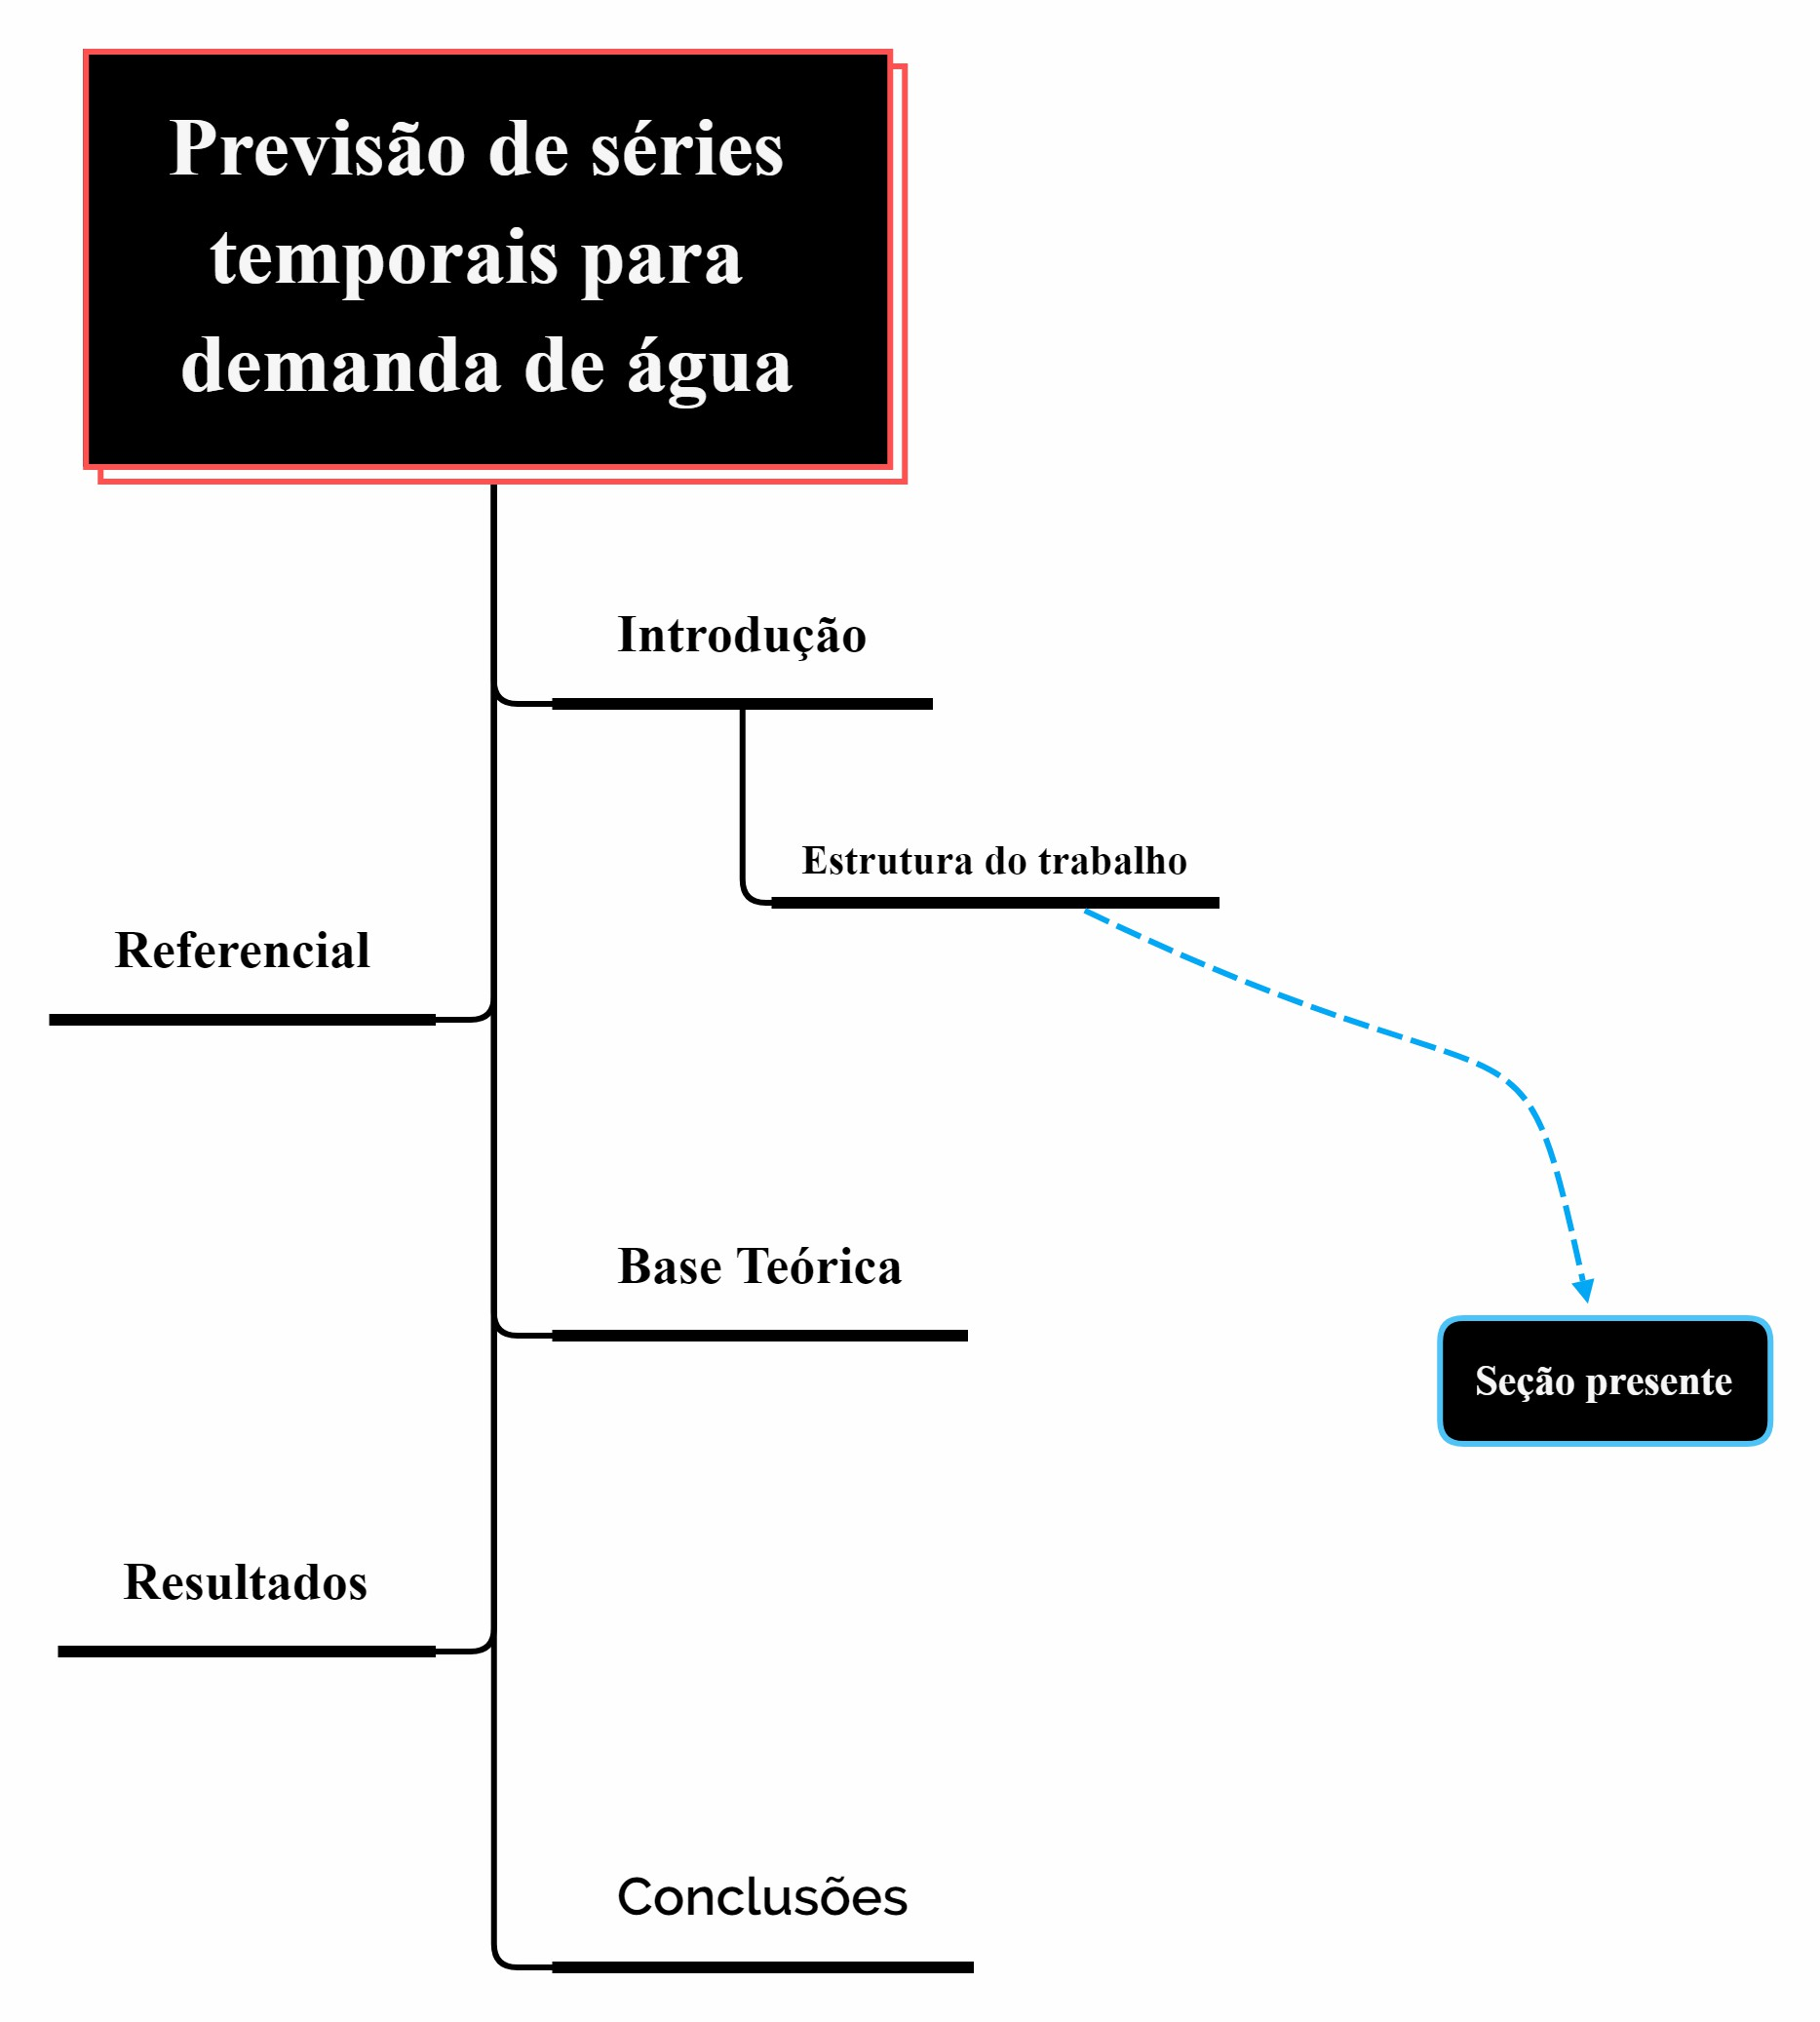
\includegraphics[width=0.9\linewidth]{Introducao/Figuras/Estrutura}
    	
    	Fonte: Elaboração própria 
    \end{figure}
%O capítulo~\ref{sec:int} apresenta a introdução do trabalho, contendo a contextualização, a motivação, o objetivo geral, os objetivos específicos e a questão de pesquisa, a descrição do problema, a metodologia utilizada, a justificativa da pesquisa, as contribuições e a organização do trabalho.
%O capítulo~\ref{sec:refteo} revisão teórica do trabalho, fazendo uma visão geral dos principais pesquisadores sobre as questões abordadas na pesquisa.
%O capítulo~\ref{sec:base} apresenta os modelos que serão trabalhados nos dados coletados.
%O capítulo~\ref{sec:result} apresenta os resultados da pesquisa, assim como uma análise dos resultados gerados.
%O capítulo~\ref{sec:conclusoes}, finalmente, apresenta as considerações finais da pesquisa e algumas propostas para pesquisas futuras.

O trabalho está estruturado em diferentes capítulos, cada um abordando aspectos específicos da pesquisa. O Capítulo~\ref{sec:int}, Introdução, apresenta a introdução do trabalho, fornecendo uma contextualização do estudo, destacando a motivação e os objetivos a serem alcançados. Também são apresentados o problema em questão, a metodologia utilizada, a justificativa da pesquisa, as contribuições esperadas e a organização do trabalho.

O Capítulo~\ref{sec:refteo}, Revisão Teórica, oferece uma visão geral das principais pesquisas e estudos relacionados às questões abordadas na pesquisa. Esse capítulo proporciona uma base teórica sólida para fundamentar a análise e interpretação dos resultados.

No Capítulo~\ref{sec:base}, Modelos, são apresentados os modelos que serão utilizados para trabalhar com os dados coletados. Essa seção detalha os modelos escolhidos, destacando suas características e fundamentos teóricos.

O Capítulo~\ref{sec:result}, Resultados, é dedicado à apresentação dos resultados obtidos ao longo da pesquisa. Além disso, são realizadas análises e interpretações dos resultados, fornecendo insights relevantes para o entendimento do problema em estudo.

Por fim, o Capítulo~\ref{sec:conclusoes}, Conclusões, traz as considerações finais da pesquisa, abordando os principais achados e conclusões alcançadas. Também são apresentadas propostas para pesquisas futuras, visando expandir e aprofundar o conhecimento na área.

Essa estrutura organizada em capítulos permite uma apresentação clara e coerente do trabalho, abrangendo desde a introdução e fundamentação teórica até os resultados e conclusões finais.


